\subsection{Race Scheduling Management Screen Flow}

\begin{figure}[H]
	\centering
	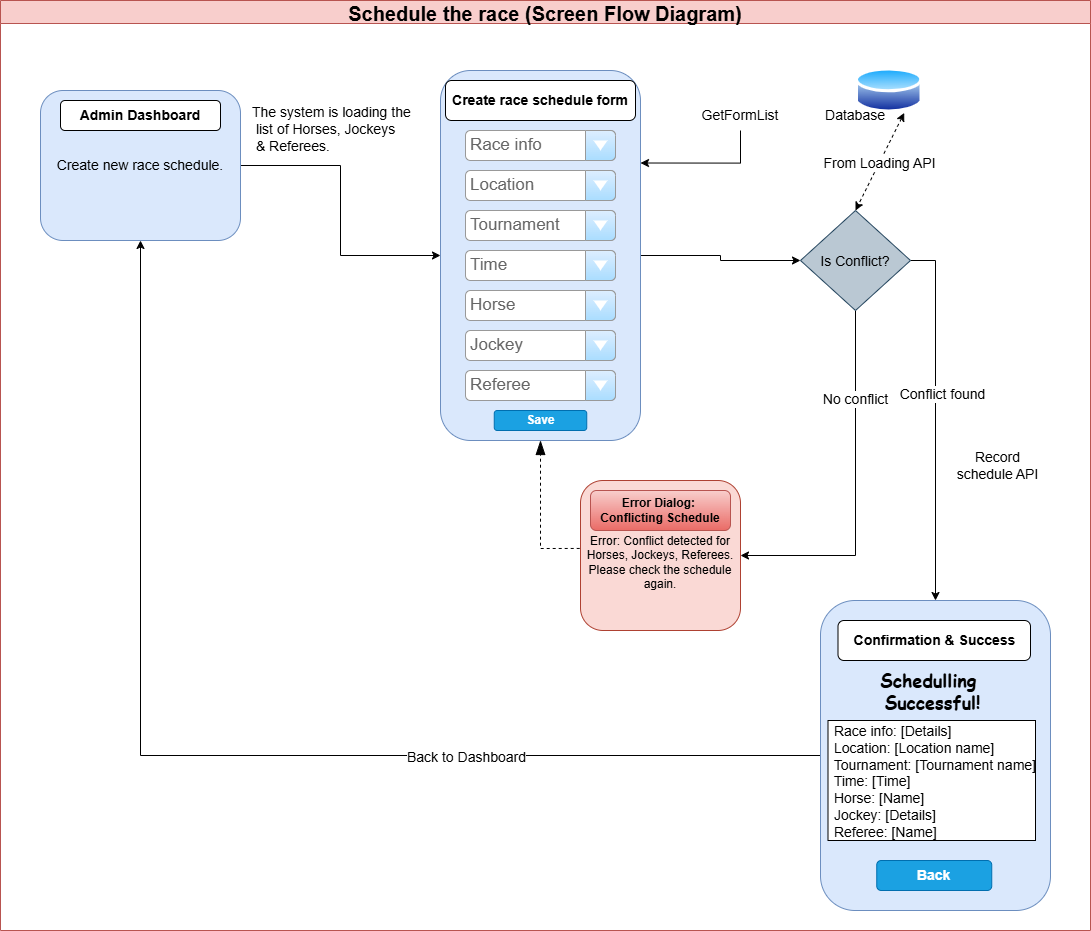
\includegraphics[width=0.9\textwidth]{figures/race_scheduling.png}
	\caption{Race scheduling management screen flow}
	\label{fig:race_scheduling_flow}
\end{figure}

\subsection{Screen description}

\begin{table}[H]
	\centering
	\begin{tabular}{|p{0.05\textwidth}|p{0.18\textwidth}|p{0.20\textwidth}|p{0.47\textwidth}|}
		\hline
		\textbf{\#} & \textbf{Feature} & \textbf{Screen} & \textbf{Description} \\
		\hline
		1 & General & Admin Dashboard & Landing page for authorized users (Admin or Referee); displays the ongoing tournament list to select a workspace. \\
		\hline
		2 & Configuration & Create Race Schedule Form & Main input interface to set up tournament stage, race name, time, track conditions, referee assignment, and lane allocation. \\
		\hline
		3 & Validation & Success Alert Banner & Prompted at the top of the form upon successful validation: Race created successfully! and appends data to the table. \\
		\hline
		4 & Validation & Invalid Time Alert & Validation error state triggered if the selected race time falls outside the tournament start and end date boundaries. \\
		\hline
		5 & Validation & Lane Conflict Alert & Validation error state triggered if multiple horses are mistakenly assigned to the same lane number. \\
		\hline
		6 & Validation & Duplicate Horse Alert & Validation error state triggered if a horse is selected more than once within the same race setup. \\
		\hline
		7 & Validation & Referee Conflict Alert & Validation error state triggered if the assigned referee has another active commitment within a 2-hour window. \\
		\hline
		8 & Feedback & Match Schedule Table & Persistent historical data table below the form showing the updated list of scheduled and completed races. \\
		\hline
	\end{tabular}
	\caption{Race Scheduling screen descriptions}
	\label{tab:raceschedulingscreens}
\end{table}